\section{\SecAdvanceNesting} \label{sec:nest_exp}
%====================================================================================

本節では、\scalerm でネスティング実験を行う方法について説明する。
ネスティングとは、水平格子間隔の異なる複数の計算領域を
領域が重複するように入れ子(ネスト)構造に設定する計算領域設定方法である。
図\ref{fig_nestsample}では、3つの領域を用いた3段ネスティングの例を示している。
外側の領域は、大きな空間スケールの現象を表現するため、低い水平解像度で広い領域を設定し、
内側の領域は、細かい現象を解像するために、狭い範囲であるが高い水平解像度に設定する。
内側の領域は、外側の領域の計算結果を境界値データとして用いる。
ここでは、入れ子構造のうち、
データを渡す側の領域を「親領域」、データを受ける側の領域を「子領域」と呼ぶことにする。

ネスティングの手法として、下記の種類に分けることができる。
\begin{itemize}
\item 実行方法
\begin{description}
 \item[オンライン・ネスティング]\mbox{}\\
親領域と子領域の計算を同時に実行し、
計算の途中で、親領域のデータを子領域へMPI通信によって受け渡しすることで、子領域の境界データを更新する方法。
 \item[オフライン・ネスティング]\mbox{}\\
まず最初に親領域の時間積分を行う。そのあと、親領域の計算結果を用いて
子領域用の初期値・境界値を作成し、子領域の時間積分を行う方法。
\end{description}
\item データの受け渡し方法
\begin{description}
 \item[一方向ネスティング]\mbox{}\\
親領域のデータは子領域に受け渡されるが、子領域の計算結果は親領域に渡されない。
つまり、データの流れは親領域から子領域に向かう一方通行。親領域は子領域の結果の影響を受けない。
 \item[双方向ネスティング]\mbox{}\\
親領域のデータは子領域へ、子領域の計算結果は親領域にフィードバックされる。
親領域の計算に、子領域の計算結果が反映される。
\end{description}
\end{itemize}

オンラインとオフラインの違いは、子領域の境界条件に与えられる親領域の情報の更新頻度にある。
\scalerm はオフライン・ネスティング実験とオンライン・ネスティング実験の両方をサポートしている。
オンラインの場合、
子領域の境界条件の更新は親領域のタイムステップ($\Delta t$) 毎に行われるが、
オフラインの場合、親領域のhitoryファイルの出力間隔に依存する。
一方、データの受け渡し方法は、\scalerm v{\version} では一方向ネスティングのみをサポートしている。

親領域と子領域の間の格子間隔の比($DX_{parent}/DX_{child}$)は、
オフライン、オンラインに関わらずシステム上の制限はないが、
この比率が大きすぎると計算結果の物理的なパフォーマンスが下がる可能性がある。
\scalerm では5倍以下で使用することを推奨する。

本節、以降の説明では、
親領域の設定ファイルを\verb|***.parent.conf| 、
子領域の設定ファイルを\verb|***.child.conf| と表記する。

\\
\proofcomment{青字と赤字の使い分けのポリシーを一貫してください。これは全文書に渡って。。。
赤字は、「かなり注意」と言う意味と思いますが、青字はどういうポリシーでしょうか?}\\
\replycomment{基本的に青字は使わないことにします。使う場合には、青字は〇〇を意味するというように、説明を入れることにします(足立)}
\proofcomment{了解。最終レビューで確認します。本件明記,残}
\\

\begin{figure}[t]
\begin{center}
  
\includegraphics[width=1.0\hsize]{./figure/nesting_sample.eps}\\
  \caption{日本の近畿地方を対象領域とした領域ネスティング設定の例。 
    domain 1が最外領域でdomain 3が最内領域である。
    赤い矩形と線は、それぞれの位置関係を示している。domain 1の水平格子間隔は7.5 km、domain 2は2.5 km、
    そしてdomain 3は0.5 kmである。}
  \label{fig_nestsample}
\end{center}
\end{figure}


\proofcomment{青字と赤字の使い分けのポリシーを一貫してください。これは全文書に渡って。。。
赤字は、「かなり注意」と言う意味と思いますが、青字はどういうポリシーでしょうか?}\\
\replycomment{基本的に青字は使わないことにします。使う場合には、青字は〇〇を意味するというように、説明を入れることにします(足立)}


\subsection{\SubsecOflineNesting} \label{subsec:nest_offline}
%------------------------------------------------------

オフラインネスティング実験を行う上での実験設定の制限事項は、以下の2点である。
\begin{itemize}
 \item 子領域の計算範囲は、親領域の計算範囲の内側に位置している必要がある。
 \item 子領域の積分期間は、親領域の積分期間と同じもしくはそれより短い必要がある。
\end{itemize}

また、オフライン・ネスティング実験の実行過程は次のようになる。
{\gt
\begin{enumerate}
 \item 親領域の時間積分計算を行う。
 \item 親領域のhistory出力ファイルを用いて子領域の初期値/境界値を作成する。
 \item 作成した初期値/境界値を用いて子領域の時間積分計算を行う。
\end{enumerate}
}

以下、この流れに沿って説明を進める。
親領域と子領域それぞれについて、\verb|pp.***.conf|、\verb|init.***.conf|、
そして\verb|run.***.conf|ファイルを事前に作成し、
親領域、子領域ともに地形・土地利用データの作成 (\verb|scale-rm_pp|) が、
親領域については、初期値/境界値データの作成 (\verb|scale-rm_ini|) が終わっていることを想定して説明を進める。
ここで説明するオフライン・ネスティング実験の設定を記述した設定ファイルが
チュートリアルディレクトリ\verb|${Tutorial_dir}/real/sample/offline_nesting|
に置いてあるので、説明を読み進める上で参考にしてもらいたい。

\subsubsection{親領域の時間積分計算を行う}
基本的には通常のシングルドメインの場合と同じ方法で実行すればよいが、
\verb|run.***.conf|の設定で次の5点に注意する必要がある。

\begin{itemize}
 \item 子領域の計算に必要な変数全てを、親領域のhistory出力。
 \item 親領域のhistory出力間隔を適度に細かくとること。
 \item 親領域のhistory出力データは、モデル面のデータを出力すること。
 \item 親領域の計算領域を子領域へ伝える「カタログファイル」(以下参照のこと)を出力する。
 \item (子領域の計算開始時刻が親領域と同じ場合) 親領域のhistory出力データにt=0の値を含めること。
\end{itemize}


この設定を\verb|run.parent.conf|に適用すると下記のようになる。\textcolor{red}{赤文字}で示した部分が、上記の注意点・変更点に対応する部分である。\\

\noindent {\small {\gt
\ovalbox{
\begin{tabularx}{140mm}{lX}
\verb|&PARAM_DOMAIN_CATALOGUE| & \\
\textcolor{red}{\verb| DOMAIN_CATALOGUE_OUTPUT = .true.,|} & カタログファイルを出力する。\\
\verb|/| &\\
 & \\
\verb|&PARAM_HISTORY| &\\
\verb| HISTORY_DEFAULT_BASENAME  = "history",| & \\
\textcolor{red}{\verb| HISTORY_DEFAULT_TINTERVAL = 600.D0,|} & historyデータの出力時間間隔。\\
\verb| HISTORY_DEFAULT_TUNIT     = "SEC",|   & \verb|HISTORY_DEFAULT_TINTERVAL|の単位。\\
\verb| HISTORY_DEFAULT_TAVERAGE  = .false.,| & \\
\verb| HISTORY_DEFAULT_DATATYPE  = "REAL4",| & \\
\textcolor{red}{\verb| HISTORY_DEFAULT_ZINTERP   = .false.,|} & モデル面データを出力。\\
\textcolor{red}{\verb| HISTORY_OUTPUT_STEP0      = .true.,|}  & t=0の値を出力に含める。 \\
\verb|/| \\
\end{tabularx}
}}}\\

カタログファイルの出力設定を\verb|.true.|にすると、\verb|latlon_domain_catalogue.txt|というカタログファイルが出力される。
この中には、親領域の計算で各MPIプロセスが担当する計算領域の四隅の緯度・経度が記述されている。
\nmitem{HISTORY_DEFAULT_TINTERVAL}はhistoryデータの出力間隔を示し、
子領域の側面境界条件を更新したい時間間隔に設定すること。
短い時間間隔でデータを出力する場合には、ディスク空き容量に注意されたい。

\\
\proofcomment{上記、HISTORY\_DEFAULT\_TUNIT  = "SEC"と書いてありますが、
秒しか許されないのでしょうか?}
%\replycomment{"sec"以外もOK。「単位は秒である」という記述は削除しました(足立)}
\\

また、子領域の初期値/境界値データ作成に必要な変数全てを
\verb|run.parent.conf|ファイルの\namelist{HISTITEM}に追加しておく必要がある。
オフライン・ネスティングに必要な変数は、下記の通りである。

\begin{alltt}
  T2, Q2, MSLP, DENS, MOMZ, MOMX, MOMY, RHOT
  LAND_SFC_TEMP, URBAN_SFC_TEMP, OCEAN_SFC_TEMP
  OCEAN_ALB_LW, OCEAN_ALB_SW, LAND_ALB_LW, LAND_ALB_SW
  OCEAN_TEMP, OCEAN_SFC_Z0M, LAND_TEMP, LAND_WATER
{\small (親の雲微物理モデルに合わせて出力; 例えばTomita08なら全て)}
  QV, QC, QR, QI, QS, QG
{\small (親の雲微物理モデルに合わせて出力; 例えばTomita08なら不要)}
  NC, NR, NI, NS, NG
\end{alltt}

設定が完了したら、\verb|scale-rm|を実行して親領域の時間積分計算を行う。

%-------------------------------------------------------------
\subsubsection{親領域の出力ファイルを用いて子領域の初期値/境界値を作成する}
次に、計算が終わった親領域のhistoryデータを用いて、子領域の初期値/境界値を作成する。
実行するプログラムは、通常の初期値/境界値作成と同じ \verb|scale-rm_init| だが、
\verb|init.child.conf|を下記のように設定する。\\

\noindent {\small {\gt
\ovalbox{
\begin{tabularx}{140mm}{lX}
\verb|&PARAM_MKINIT_REAL| &\\
\verb| BASENAME_BOUNDARY   = "boundary",| &\\
\textcolor{red}{\verb| BASENAME_ORG        = "history",|}  & \verb|run.parent.conf|の\verb|HISTORY_DEFAULT_BASENAME|\\
\textcolor{red}{\verb| FILETYPE_ORG        = "SCALE-RM",|} & \\
\textcolor{red}{\verb| NUMBER_OF_TSTEPS    = 25,|}         & historyファイル内の時間ステップ数\\
\textcolor{red}{\verb| BOUNDARY_UPDATE_DT  = 600.D0,|}     & historyファイルの出力時間間隔(単位は秒)\\
\verb|/| &\\
 & \\
\textcolor{red}{\verb|&PARAM_NEST|} & \\
\textcolor{red}{\verb| USE_NESTING               = .true.,|} & \\
\textcolor{red}{\verb| OFFLINE                   = .true.,|} & \\
\textcolor{red}{\verb| OFFLINE_PARENT_PRC_NUM_X  = 4,|}  & \verb|run.parent.conf|の\verb|PRC_NUM_X|\\
\textcolor{red}{\verb| OFFLINE_PARENT_PRC_NUM_Y  = 4,|}  & \verb|run.parent.conf|の\verb|PRC_NUM_Y|\\
\textcolor{red}{\verb| OFFLINE_PARENT_KMAX       = 35,|} & \verb|run.parent.conf|の\verb|KMAX|\\
\textcolor{red}{\verb| OFFLINE_PARENT_IMAX       = 40,|} & \verb|run.parent.conf|の\verb|IMAX|\\
\textcolor{red}{\verb| OFFLINE_PARENT_JMAX       = 40,|} & \verb|run.parent.conf|の\verb|JMAX|\\
\textcolor{red}{\verb| OFFLINE_PARENT_LKMAX      = 5,|}  & \verb|run.parent.conf|の\verb|LKMAX|\\
\textcolor{red}{\verb| LATLON_CATALOGUE_FNAME    = "latlon_domain_catalogue.txt",|} & 親領域を実行した時に作成したカタログファイル\\
\textcolor{red}{\verb|/|} &\\
\end{tabularx}
}}}\\


\scalerm の出力データから初期値境界値を作成する場合は、\nmitem{FILETYPE_ORG}に\verb|SCALE-RM|を指定する。
\nmitem{BOUNDARY_UPDATE_DT}は、基本的に、親領域の設定ファイル(\verb|run.parent.conf|)の
\nmitem{HISTORY_DEFAULT_TINTERVAL}と同じ設定を記述する。
%
\namelist{PARAM_NEST}の項目は、ネスティング実験のための設定項目である。
オフライン・ネスティングでは、\nmitem{USE_NESTNG=.true., OFFLINE=.true.}と設定する。
\nmitem{OFFLINE_PARENT_**} で始まる6つの設定変数は親領域の設定を記述する変数である。
親領域の設定ファイル(\verb|run.parent.conf|) を参照して正しく設定すること。


設定の編集が完了したら、\verb|scale-rm_init|を実行し、子領域の初期値/境界値を作成する。\\

\noindent {\small {\gt
\fbox{
\begin{tabularx}{140mm}{l}
\verb|xxx ERROR: REQUESTED DOMAIN IS TOO MUCH BROAD| \\
\verb|xxx -- LONGITUDINAL direction over the limit| \\
\end{tabularx}
}}}\\

\noindent 実行時に上記のようなメッセージが表示されて計算が止まる場合は、
子領域の計算領域が親領域の計算領域の外側に取られている部分がある。
この場合は、各領域の大きさや領域中心の設定を見直す必要がある。


\subsubsection{作成した初期値/境界値を用いて子領域の時間積分計算を行う}
初期値/境界値作成が終わったら、子領域の計算 (\verb|scale-rm|) を実行する。
子領域の実行は、通常の現実大気実験と同じである。
1点だけ注意すべき点として、
\verb|run.child.conf|の\namelist{PARAM_MKINIT_REAL}の\nmitem{BOUNDARY_UPDATE_DT}を、
初期値/境界値作成で使用した親領域のhistoryデータ出力間隔に合っているか確認すること。
現在のところ、この設定に親領域と子領域間で不整合あっても警告やエラーメッセージが発せられないまま、
計算が進み、場合によっては正常終了してしまうため注意が必要である。


\noindent {\small {\gt
\ovalbox{
\begin{tabularx}{140mm}{l}
\verb|&PARAM_MKINIT_REAL| \\
\verb|     〜 中略 〜|\\
\textcolor{red}{\verb| BOUNDARY_UPDATE_DT  = 600.D0,|} \\
\verb|/| \\
\end{tabularx}
}}}\\

\noindent 

多段のオフライン・ネスティング実験を行いたい場合は、以上の過程を繰り返せばよい。
つまり、子領域として時間積分計算した結果を再度、親領域と見立てて、
さらに内側の孫領域の初期値/境界値作成を行なえばよい。



\subsection{\SubsecOnlineNesting} \label{subsec:nest_online}
%------------------------------------------------------

オンライン・ネスティング実験の場合、
現在のところ、親領域と子領域の積分時間は一致している必要があり、
かつ、親領域の時間ステップは子領域の時間ステップの倍数でなければならない。
\scalerm ではオンライン・ネスティングであっても、
親領域と子領域の間で鉛直層数、鉛直層設定、地図投影法、そして
物理スキームが異なっていても構わない。

オフライン・ネスティング実験では、各領域の計算を逐次的に実行する必要があったが、
オンライン・ネスティング実験では全ての領域の計算を同時に実行する。
現在は、親領域から子領域へのみデータ受け渡しを行う、いわゆる
``1-wayネスティング''のみをサポートしている。
オンライン・ネスティング実験でサポートするネスティング段数は、最大で10段までである。

\scalerm のオンライン・ネスティング実験は、
複数の領域を逐次的に時間積分計算を進めるのではなく、並列的に時間積分計算を行う。
図\ref{fig_mpisplit}に示すイメージ図のように、
与えられたMPIプロセスを分割してそれぞれの領域に分配し、
各々の領域が独立したモデルのように計算を進める。
後ほど説明するが、複数の領域を立ち上げるために実行時には``launch.conf''という
起動用の設定ファイルが別途必要になる。

\begin{figure}[t]
\begin{center}
  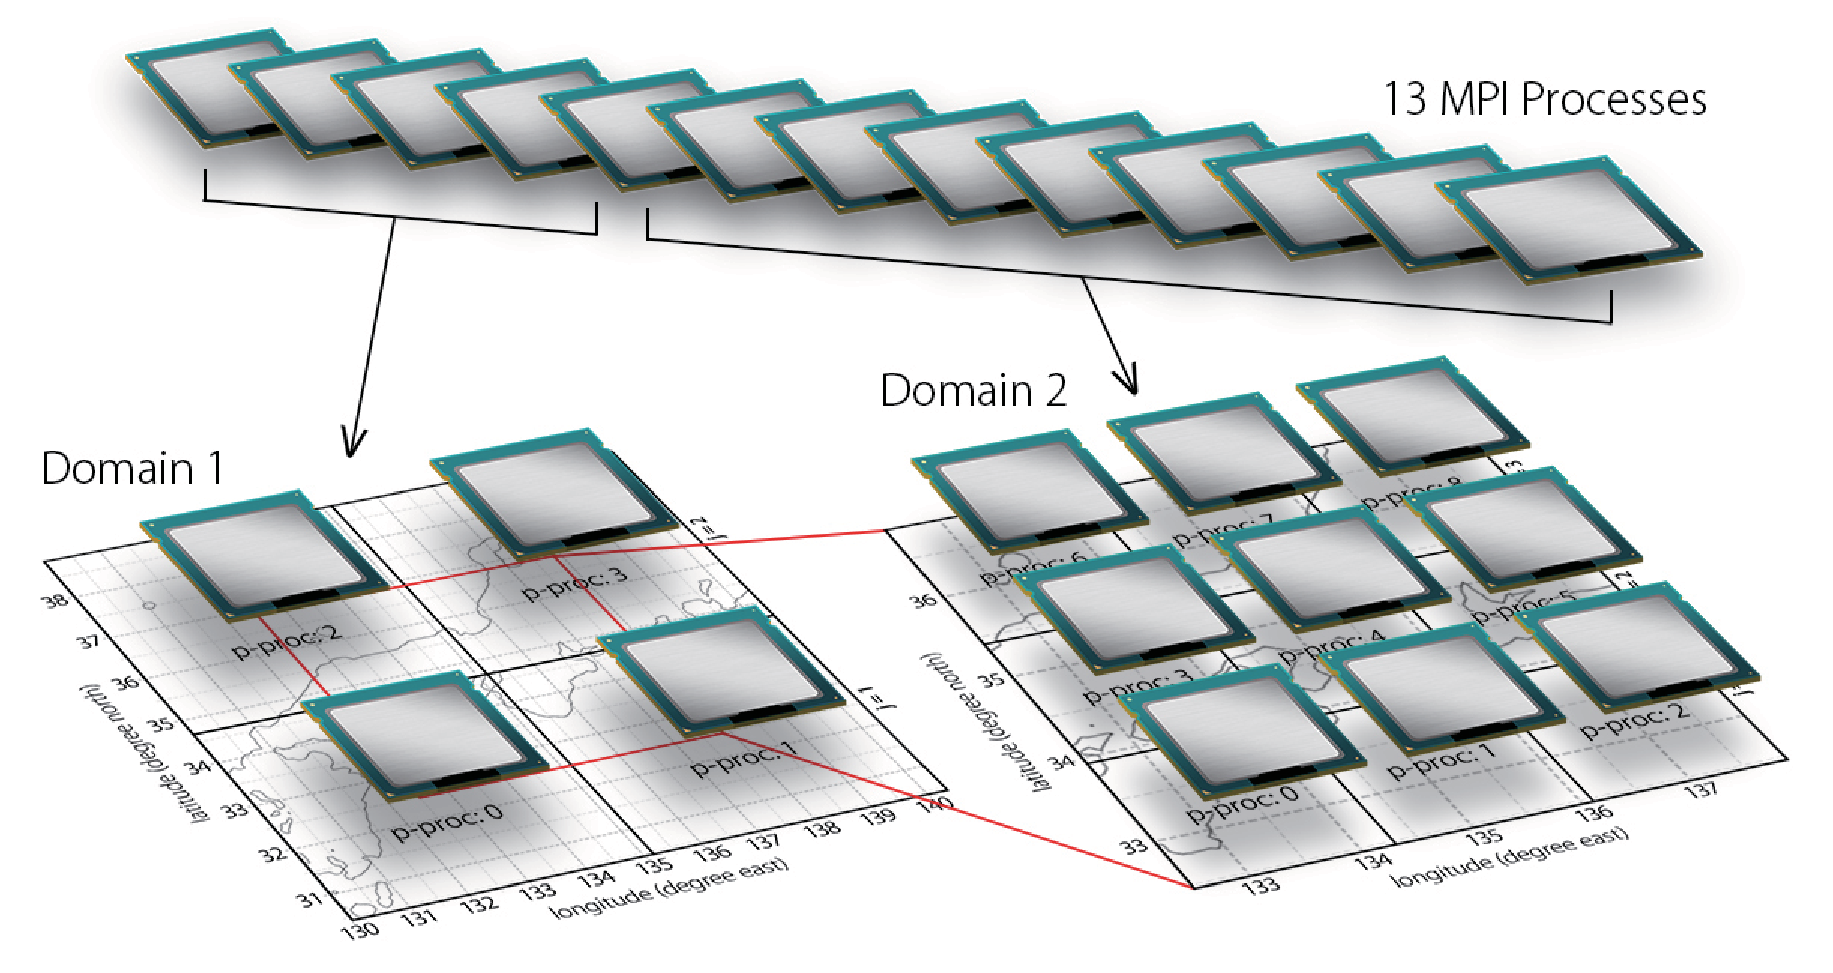
\includegraphics[width=0.8\hsize]{./figure/mpisplit_nesting.eps}\\
  \caption{オンライン・ネスティング実験のMPIプロセス配分イメージ. 全部で13のプロセスを立ち上げ、これを適切に分配することで、
           Domain 1は$2 \times 2$の4-MPI並列、Domain 2は$3 \times 3$の9-MPI並列計算を行う。Domain 1からDomain 2へMPI通信
           によってデータを受け渡ししながら時間積分計算を進める。}
  \label{fig_mpisplit}
\end{center}
\end{figure}


ここでは、最も単純な2段ネスティングの例を説明する。親領域は解像度は粗いが広領域の外側領域で、
子領域は領域は狭いが高解像度の内側領域であることを想定する。
オンライン・ネスティング実験を行う場合は、``scale-rm''のモデル本体実行前に全ての領域について、
地形/土地利用データの作成、及び初期値/境界値データの作成を事前に行っておく必要がある。
従って、親領域と子領域それぞれについて、
``pp.***.conf''、``init.***.conf''、そして``run.***.conf''ファイルを事前に作成し、
親領域、子領域ともに地形/土地利用データの作成、
及び初期値/境界値データの作成を終えていることを想定して説明を進める。
ここで説明するオンライン・ネスティング実験の設定を記述した設定ファイルがチュートリアルディレクトリの下、
\verb|${Tutorial_dir}/real/sample/online_nesting|に置いてあるので、
説明を読み進める上で参考にしてもらいたい。


\subsubsection{設定ファイルの編集}
まず、親領域、子領域それぞれに``run.***.conf''ファイルを編集する。

\noindent {\gt \verb|run.parent.conf|の編集内容}\\
{\small {\gt
\ovalbox{
\begin{tabularx}{140mm}{l}
\verb|&PARAM_NEST| \\
\verb| USE_NESTING              = .true.,| \\
\verb| OFFLINE                  = .false.,| \\
\verb| ONLINE_DOMAIN_NUM        = 1,| \\
\verb| ONLINE_IAM_PARENT        = .true.,| \\
\verb| ONLINE_IAM_DAUGHTER      = .false.,| \\
\verb| ONLINE_BOUNDARY_USE_QHYD = .true.,| \\
\verb| ONLINE_AGGRESSIVE_COMM   = .true.,| \\
\verb|/| \\
\end{tabularx}
}}}\\

\vspace{0.5cm}

\noindent {\gt \verb|run.child.conf|の編集内容}\\
{\small {\gt
\ovalbox{
\begin{tabularx}{140mm}{l}
\verb|&PARAM_NEST| \\
\verb| USE_NESTING              = .true.,| \\
\verb| OFFLINE                  = .false.,| \\
\verb| ONLINE_DOMAIN_NUM        = 2,| \\
\verb| ONLINE_IAM_PARENT        = .false.,| \\
\verb| ONLINE_IAM_DAUGHTER      = .true.,| \\
\verb| ONLINE_BOUNDARY_USE_QHYD = .true.,| \\
\verb| ONLINE_AGGRESSIVE_COMM   = .true.,| \\
\verb|/| \\
\end{tabularx}
}}}\\

\noindent 上記の\namelist{PARAM_NEST}の項目は、ネスティング実験のために新たに加える項目である。
もともとの設定ファイルには項目自体がないので、自分で設定ファイルに追記する。最初の2つの項目
\nmitem{USE_NESTING = .true., OFFLINE = .false.}によって、
オンライン・ネスティング実験であることが決定される。
\nmitem{ ONLINE_}で始まる設定変数はオンライン・ネスティング実験
専用の設定変数である。\nmitem{ONLINE_DOMAIN_NUM}は、
領域のID番号であり、外側領域から内側領域へ順番に
番号を振っていく。ここでは、親領域は1番、子領域は2番と設定する。

\nmitem{ONLINE_IAM_PARENT}と\nmitem{ONLINE_IAM_DAUGHTER}は各領域の役割を設定するパラメータである。
これらの変数は、``In online nesting system, I am parent (or, I am child).''という意味で覚えれば設定を間違うことはない。
少し脇道にそれるが、
ここで説明している設定より複雑なものとして、図\ref{fig_nestsample}のような
3段ネスティング実験の場合の設定例を表\ref{tab:triple_nested}に示した。

\begin{table}[htb]
\begin{center}
\caption{3段ネスティング実験の設定例}
\begin{tabularx}{150mm}{|l|l|l|X|} \hline
 \rowcolor[gray]{0.9} 領域 & \verb|ONLINE_DOMAIN_NUM| & \verb|ONLINE_IAM_PARENT| & \verb|ONLINE_IAM_CHILD|\\ \hline
 最外領域 & 1 & \textcolor{blue}{true} & \textcolor{red}{false} \\ \hline
 中間領域 & 2 & \textcolor{blue}{true} & \textcolor{blue}{true} \\ \hline
 最内領域 & 3 & \textcolor{red}{false} & \textcolor{blue}{true} \\ \hline
\end{tabularx}
\label{tab:triple_nested}
\end{center}
\end{table}

\noindent 最外領域は親領域としてのみ働き、最内領域は子領域としてのみ働く。
一方、中間領域は最外領域に対しては子領域、
最内領域に対しては親領域として働くため両方共``true''となる。

さて、設定ファイルの編集内容の説明に戻る。\nmitem{ONLINE_BOUNDARY_USE_QHYD}は、
「側面境界条件として親領域の凝結物の混合比を使うかどうか」を指定する設定変数である。
外部入力データから側面境界条件を作成するときには通常使わないが、
ネスティングの場合、領域間の物理スキームの違いがなかったり、
解像度もそれほど大きく離れていないため、
側面境界から
凝結物自体が移流して入ってくる設定も選択肢に入るだろう。
側面境界付近で雲が立ちにくい問題を解決したり、親領域との乖離を抑制したりする働きがある。

%最後の\verb|ONLINE_AGGRESSIVE_COMM|はオンライン・ネスティング時の領域間通信に関する最適化変数である。
%通常は、``true''と設定して実行する。


\subsubsection{launchファイルの編集}
オンライン・ネスティング実験の実行には、``run.***.conf''の他に、起動用設定ファイル``launch.conf''が必要である。
以下のような新規ファイルを作成する。\\

\noindent {\small {\gt
\ovalbox{
\begin{tabularx}{140mm}{l}
\verb|&PARAM_LAUNCHER| \\
\verb| NUM_DOMAIN  = 2,| \\
\verb| CONF_FILES  = run.parent.conf,run.child.conf,| \\
\verb| PRC_DOMAINS = 4,9,| \\
\verb|/| \\
\end{tabularx}
}}}\\

\noindent 図\ref{fig_mpisplit}のイメージを思い浮かべながら設定を確認してもらいたい。
\namelist{PARAM_LAUNCHER}の項目のうち、
\nmitem{NUM_DOMAIN = 2}が「2つの領域を起動する」ことを表しており、
\nmitem{CONF_FILES}の項目に羅列されたファイル名は、
各々の領域で読み込む設定ファイルを指定している。
\nmitem{PRC_DOMAINS}は各々の領域で使用するMPIプロセス数を
指定する。
\nmitem{PRC_DOMAINS}は、
\nmitem{CONF_FILES}で羅列した順番で指定しなければならない。従ってこの場合、
親領域は4-MPI並列、
子領域は9-MPI並列で実行するように指定されている。ここで指定するMPIプロセス数は、
各々の``run.***.conf''で指定されている総MPIプロセス数と合致させなければならない。
この2段オンライン・ネスティング実験で使用する総MPIプロセス数は、$4 + 9 = 13$プロセスとなる。

実行時には、シングル領域計算とは異なり、\verb|launch.conf|を引数に指定し、計算全体で使用するMPIプロセス数を
指定して実行する。
\begin{verbatim}
 $ mpirun  -n  13  ./scale-rm  launch.conf
\end{verbatim}

実行にあたって注意することは、複数の領域の計算を同時に実行するため、\textcolor{red}{領域間で設定ファイルに
記述された出力ファイル名を領域毎に変更しなければならない}ことである。たとえば,``history.pe***.nc''は、
``history\_d01.pe***.nc''、``history\_d02.pe***.nc''といったように領域毎に名前を変えながらどの領域の
出力データであるか判別がつくように設定ファイルの記述を設定する。
historyファイルのほかに、LOGファイル、topoファイル、landuseファイル、boundaryファイル、initファイル、restartファイル、
そしてmonitorファイルの名前を変更しておく必要がある。

実行時に次のようなエラーメッセージが出力されて計算が異常終了することがある。\\

\noindent {\small {\gt
\fbox{
\begin{tabularx}{140mm}{l}
\verb|xxx region of daughter domain is larger than that of parent: SW search| \\
\end{tabularx}
}}}\\

\noindent {\small {\gt
\fbox{
\begin{tabularx}{140mm}{l}
\verb|xxx region of daughter domain is larger than that of parent: NE search| \\
\end{tabularx}
}}}\\

\noindent これは、子領域で設定された計算領域が親領域の計算領域よりも大きいことを意味するエラーメッセージである。
``SW search''のエラーが出る場合は子領域の西側か南側が親領域の外側に出ており、``NE search''のエラーが出る場合は
子領域の東側か北側が親領域の外側に出ていることを意味している。再度設定を確認し、地形・土地利用データ、および
初期値/境界値作成からやり直すこと。


\subsubsection{MPIプロセスの分配ガイドライン}
SCALE-RMのオンライン・ネスティング実験は、図\ref{fig_mpisplit}のイメージ図で説明したように、MPIプロセスを分割し、複数の領域
に分配する。現在のところ、その分配割合はユーザーに委ねられているため、適切にMPIプロセスを分配しなければ余計な計算時間が
かかってしまう。ここでは、適切にMPIプロセスを分配するためのガイドラインについて説明する。ガイドラインは、領域毎に
\textcolor{blue}{「単位あたりの時間積分にかかる1プロセスあたりの演算量を揃える」}という単純なものである。
ここでは、以下に示す2段オンライン・ネスティング実験を行う場合を想定し、ガイドラインに沿ったプロセス分配方法の例を示す。
``domain 1''は外側の親領域、``domain 2''は内側の子領域を意味する。

\begin{table}[htb]
\begin{center}
\caption{2段オンライン・ネスティング実験の設定想定}
\begin{tabularx}{150mm}{|l|l|X|} \hline
 \rowcolor[gray]{0.9} 設定項目 & domain 1 & domain 2 \\ \hline
 計算領域 & 450 km $\times$ 450 km & 200 km $\times$ 200 km \\ \hline
 DX \& DY(X,Y同一設定) & 3 km & 1 km \\ \hline
 鉛直層設定 & 40層 & 60層 \\ \hline
 積分時間間隔(DT)& 30 sec & 10 sec \\ \hline
 積分時間 & 3600 sec & 3600 sec \\ \hline
\end{tabularx}
\label{tab:nest_proc_guide1}
\end{center}
\end{table}

このとき、親領域の水平方向の一辺の格子点数は、$450 \mathrm{km} \div 3 \mathrm{km} = 150$点であるので、総格子点数は
$X \times Y \times Z = 150 \times 150 \times 40 = 900,000$点である。一方、子領域の水平方向の一辺の格子点数は、
$200 \mathrm{km} \div 1 \mathrm{km} = 200$点であるので、
総格子点数は$200 \times 200 \times 60 = 2,400,000$点である。1つの時間ステップの
積分を行うのにこれだけの格子点について計算を行わなければならない。

積分時間間隔は格子間隔に依存するために領域毎に異なる。この例では、domain 1は30 secだが、domain 2は10 secであり、
3倍の差がある。したがって、同じ30 secという積分時間に対してdomain 2は3倍多くの時間ステップ、つまり3倍の演算量を要する。
これらを考慮して、簡単な領域間の演算量比率(Computation Rate)の指標を考えると下記の式で表される。
\begin{eqnarray}
ComputationRate=\frac{Xgrd_{child} \times Ygrd_{child} \times Zgrd_{child} \times Ustep_{child}}
                     {Xgrd_{parent} \times Ygrd_{parent} \times Zgrd_{parent} \times Ustep_{parent}} \nonumber
\end{eqnarray}
ここで、$Xgrd, Ygrd, Zgrd$ はそれぞれ{\XDIR} 、{\YDIR}、{\ZDIR}の格子点数を表し、Ustepは単位時間積分に必要な時間ステップ数を表す。
ここでの例をこの式に当てはまると、
演算量比率は$(2,400,000 \times 3) \div (900,000 \times 1) = 8$であることがわかる。
おおよそ、この割合にしたがってMPIプロセスを領域毎に分配すればよい。
例えばdomain 1は4プロセス、domain 2は32プロセスを
使用し、全体で36プロセスを使用する設定が考えられる。
この場合、例えば次のように設定することができる。

\begin{table}[htb]
\begin{center}
\caption{2段オンライン・ネスティング実験のMPIプロセス設定例}
\begin{tabularx}{150mm}{|l|l|X|} \hline
 \rowcolor[gray]{0.9} 設定項目 & domain 1 & domain 2 \\ \hline
 MPIプロセス(X $\times$ Y) & 2 $\times$ 2 & 4 $\times$ 8 \\ \hline
 水平格子点数(IMAX $\times$ JMAX) & 75 $\times$ 75 & 50 $\times$ 25 \\ \hline
\end{tabularx}
\label{tab:nest_proc_guide2}
\end{center}
\end{table}

{\XDIR} と{\YDIR}に分配するプロセス数には任意性が残るが、
IMAXとJMAXの違を小さくとる方がハロ領域を小くすることが出来るため、
計算機の演算性能を引き出しやすいと考えられる\footnote{ただし、京の場合のようにスレッド並列も併用するハイブリッド並列の場合には{\YDIR}の格子点数をある程度大きくしてスレッド間の演算量のインバランスを小さくする必要性も出てくる。}。

この設定は一例であり、
これ以外の方法で設定しても構わない。
また、ここでは格子点数と積分時間間隔だけに着目して演算量比率を考えたが、
実際の計算には様々な物理過程も含まれるだろうし、
それらを 呼び出す時間間隔も領域毎に異なるかもしれない。
さらに領域内通信や領域間通信のMPI通信にかかる時間も影響を及ぼす。
オンライン・ネスティングの設定では、
最も計算負荷が高い領域(通常は最内領域)が時間積分を実行し続ける
(MPI通信のための待ち時間が最小になる)ようにプロセスを分配するのが効率的である場合が多い。
同じ設定で何度も実験を行うような場合には、
上記の方法である程度の見通しをつけた上で、いくらかの微調整を行うことをおすすめする。
以上でオンライン・ネスティングの実行方法の説明を終える。


\subsection{子領域における地形の取り扱い} \label{subsec:nest_topo}
%------------------------------------------------------
ネスティング実験を行う際、領域間の格子間隔比率が大きい場合などに
子領域の緩和領域内で不整合が発生する
可能性がある。
緩和領域内は親領域の計算結果を用いて一部の変数を緩和していくが、地形の表現性が異なる
ことで、子領域にとっては正しくない値へ引きずられる可能性がある。
例えば、子領域では斜面上の小さな谷として
表現されている地形が、親領域では格子間隔が大きすぎて
谷がなくスムーズな斜面として表現される場合が考えられる。

こういった不整合を無くすために、緩和領域では親領域の地形を用い、内側領域では子領域自身の地形を用いる
「地形コピー」の機能が実装されている。この機能を使えば、図\ref{fig_topocopy}に示すように緩和領域は完全に
親領域に一致する地形で、内側に移る地形遷移領域内では親領域と子領域のミックス、それより内側では完全に
子領域の地形という設定を構築することができる。以降、その設定方法と実行手順を説明する。
基本的には、オフライン・ネスティングのフレームワークを利用して進める。

\proofcomment{この文書では、オンラインが推奨されています。ですのでオンラインの記述も必要かと思います。}

ここで説明する地形コピーの設定を記述した``pp.d0*.conf''ファイルがチュートリアルディレクトリ
\verb|${Tutorial_dir}/real/sample/online_nesting|に置いてあるので、
説明を読み進める上で参考にしてもらいたい。

\begin{figure}[tb]
\begin{center}
  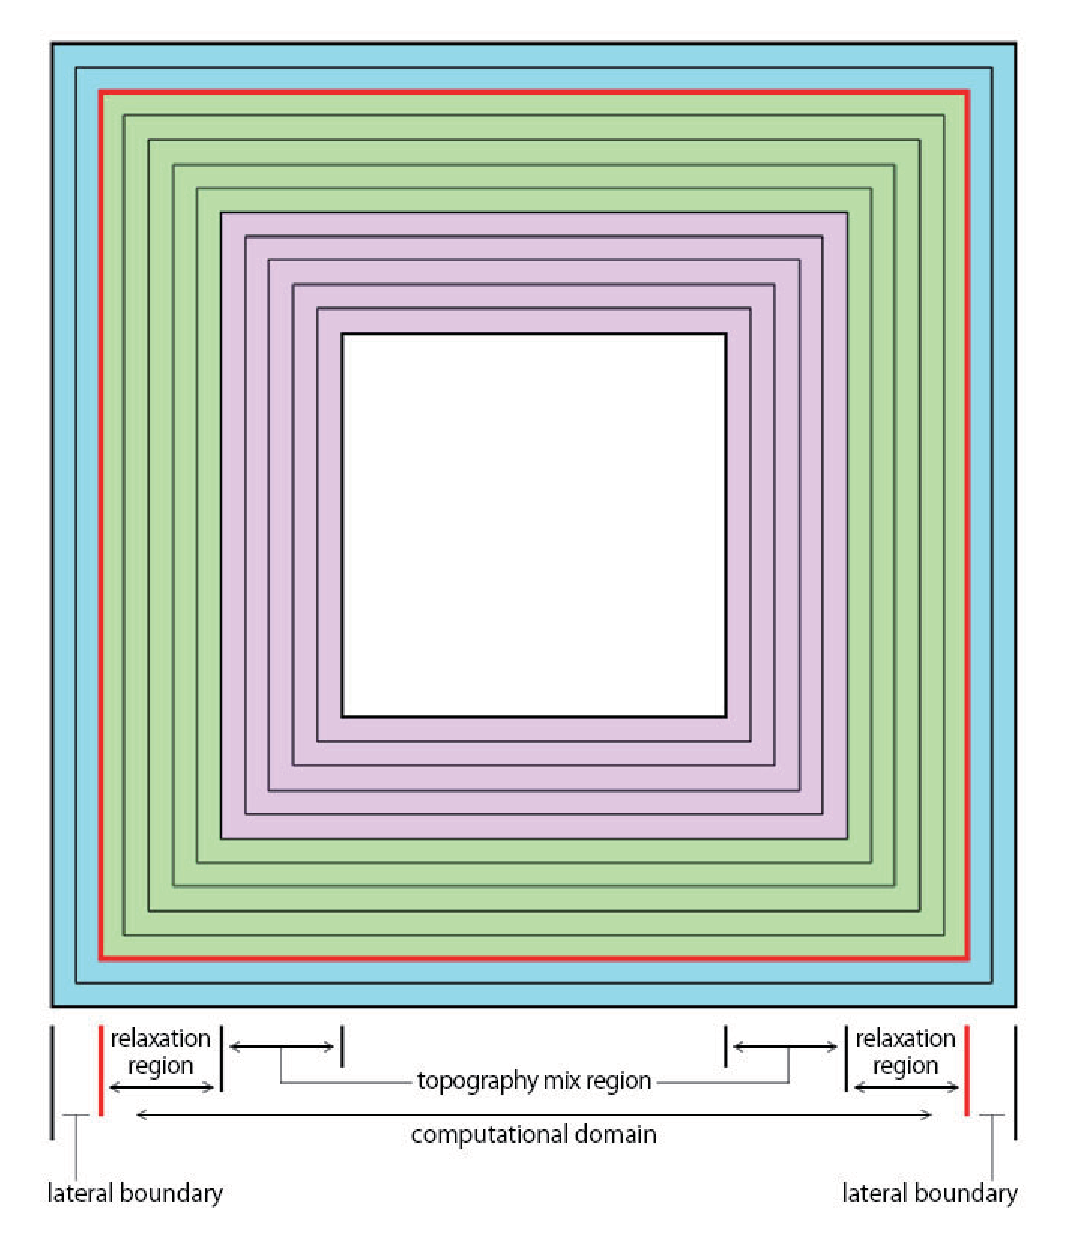
\includegraphics[width=0.4\hsize]{./figure/topo_copy.eps}\\
  \caption{地形コピーを適用した子領域の地形データ水平分布. 最外の水色の2格子(Haloの数。水平差分スキームによって異る)は側面境界で、それより内側の赤色の線で
           囲われた領域が計算領域である。緑色の部分が緩和領域、桃色の部分が地形遷移領域、そして最内の白色の
           部分が子領域の地形をもつ領域である。地形遷移領域では外側から内側にかけて徐々に親領域の地形データから
           子領域の地形データへ遷移する。}
  \label{fig_topocopy}
\end{center}
\end{figure}

まず親領域の``pp.d01.conf''ファイルを編集して、計算領域の大きさを子領域へ伝えるために緯度経度カタログ
ファイルを出力するように設定する。具体的には、下記の記述を``pp.d01.conf''ファイルに追記する。\\

\noindent {\small {\gt
\ovalbox{
\begin{tabularx}{140mm}{l}
\verb|&PARAM_DOMAIN_CATALOGUE| \\
\verb| DOMAIN_CATALOGUE_FNAME  = "latlon_domain_catalogue.txt",| \\
\verb| DOMAIN_CATALOGUE_OUTPUT = .true.,| \\
\verb|/| \\
\end{tabularx}
}}}\\

\noindent その他の設定項目は通常通りで良い。編集ができたら親領域の地形データ作成を実行する(つまり、
scale-rm\_ppを実行する)。ここで、出力データは、``topo\_d01.pe***.nc''というファイル名で保存されていると
想定する。次に、子領域の``pp.d02.conf''ファイルを編集する。\\

\noindent {\small {\gt
\ovalbox{
\begin{tabularx}{140mm}{l}
\verb|&PARAM_CNVTOPO| \\
\verb|     〜 中略 〜|\\
\verb| CNVTOPO_copy_parent     = .true.,| \\
\verb|/| \\
 \\
\verb|&PARAM_COPYTOPO| \\
\verb| COPYTOPO_IN_BASENAME   = "topo_d01",| \\
\verb| COPYTOPO_ENTIRE_REGION = .false.,| \\
\verb| COPYTOPO_LINEAR_H      = .true.,| \\
\verb|/| \\
 \\
\verb|&PARAM_NEST| \\
\verb| USE_NESTING               = .true.,| \\
\verb| OFFLINE                   = .true.,| \\
\verb| OFFLINE_PARENT_PRC_NUM_X  = 4,| \\
\verb| OFFLINE_PARENT_PRC_NUM_Y  = 4,| \\
\verb| OFFLINE_PARENT_KMAX       = 35,| \\
\verb| OFFLINE_PARENT_IMAX       = 40,| \\
\verb| OFFLINE_PARENT_JMAX       = 40,| \\
\verb| OFFLINE_PARENT_LKMAX      = 5,| \\
\verb| LATLON_CATALOGUE_FNAME    = "latlon_domain_catalogue.txt",| \\
\verb|/| \\
\end{tabularx}
}}}\\

\noindent 
地形コピーを用いるには、もともと設定ファイルにある\namelist{PARAM_CNVTOPO}の項目に、
\nmitem{CNVTOPO_copy_parent = .true.}
という記述を加える。
次の\namelist{PARAM_COPYTOPO}は、
地形コピーの設定項目群であり、すべて追記すること。
1つ目の\nmitem{COPYTOPO_IN_BASENAME}は、
親領域の地形データのPATHを指定する。ここでは、親領域の
出力データは``topo\_d01.pe***.nc''というファイル名で
カレントディレクトリに保存されていると指定している。
2つ目の\nmitem{COPYTOPO_ENTIRE_REGION}は、全領域でコピーするかどうかを決定するオプションである。
このスイッチをtrueにすると、図\ref{fig_topocopy}に示された桃色と白色の領域は無くなり、全て緑色の
完全コピー領域になる。3つ目の\nmitem{COPYTOPO_LINEAR_H}は、
地形遷移領域の遷移具合を調整するスイッチである。
\nmitem{COPYTOPO_LINEAR_H}がtrueだと線形プロファイルで遷移し、
falseだと指数関数プロファイルで遷移する。

地形遷移領域の幅は、デフォルト設定では緩和領域と同じ幅になる。緩和領域の設定と同じ要領で、
\nmitem{COPYTOPO_TRANSITION_DX}、\nmitem{COPYTOPO_TRANSITION_DY}、
および\nmitem{COPYTOPO_TRANSFACT}の
変数を使って任意の幅に設定することができる。

最後の\namelist{PARAM_NEST}の項目はオフライン・ネスティング実験の
フレームワークを利用するための設定項目であり、
全て追記する必要がある。
設定変数の詳しい説明は、\ref{subsec:nest_offline}節の
オフライン・ネスティング実験の説明を参照してほしい。

設定ファイルの編集が終われば、子領域の地形データ作成を実行する。3つ以上の領域がある場合は、
上記の実行過程を外側領域から順に繰り返せばよい。



